% Preamble
\documentclass[12pt, a4paper]{report}

% Packages
\usepackage{polski}
\usepackage[utf8]{inputenc}
\usepackage{booktabs}
\usepackage[margin=1in, footskip=0.25in]{geometry}
\usepackage{threeparttable}
\usepackage{float}
\usepackage{makecell}
\usepackage{indentfirst}
\usepackage{graphicx}
\usepackage{longtable}
\usepackage{subcaption}
\usepackage{hyperref}
\usepackage{amsmath}
\usepackage{listings}

\title{Systemy Wbudowane - AstroPi Challenge}
\author{Marcin Przewięźlikowski, Maciej Trzebiński}

% Document
\begin{document}
    \maketitle

    \tableofcontents{}

    \chapter{Wstęp}\label{ch:introduction}

    W ramach zajęć z przedmiotu Systemy Wbudowane wystartowaliśmy w konkursie Astro Pi
    Challenge. Konkurs ten jest organizowany przez Europejską Agencję Kosmiczną (ESA) i ma na celu
    promowanie wśród uczniów i studentów zainteresowania eksperymentami naukowymi. ESA udostępnia
    uczestnikom konkursu dwa mikrokomputery RaspberryPi znajdujące się na pokładzie Międzynarodowej
    Stacji Kosmicznej (ISS) do celów eksperymentu. Właściwa część eksperymentu ma skupiać się na
    monitorowaniu Ziemi lub kosmosu za pomocą czujników, w które wyposażony jest mikrokomputer przez
    czas nie przekraczający trzech godzin.

    Eksperyment został podzielony się na cztery fazy:
    \begin{itemize}
        \item[Faza 1:] Każdy zespół planuje swój eksperyment, a komisja złożona z pracowników
        ESA ocenia go i wybiera najlepsze propozycje.
        \item[Faza 2:] Zespoły, których eksperymenty zostały zaklasyfikowane do fazy 2 piszą kod eksperymentu
        i wysyłają go komisji, która ocenia, czy kod spełnia wymagania formalne.
        \item[Faza 3:] Kody pozytywnie zaopiniowane przez komisję są uruchamiane na komputerach wbudowanych na pokładzie
        ISS.
        \item[Faza 4:] Wyniki eskperymentów dostarczane są do zespołów, które mają miesiąc czasu na ich analizę i
        dostarczenie wniosków z analizy wyników.
    \end{itemize}

    Nasz zespół podjął się zadania zbadania ilości światła emitowanego z powierzchni Ziemi w nocy.
    Pozwoli to określić poziom zanieczyszczenia światłem w poszczególnych rejonach, oraz zużycie energii
    elektrycznej na sztuczne oświetlenie w krajach, w których takie dane nie są zbierane lub udostępniane,
    na podstawie takich danych udostępnionych przez innne kraje oraz zdjęć kuli ziemskiej wykonanych z pokładu ISS.

    \chapter{Skonfigurowanie platformy treningowej}\label{ch:cover}
    \section{Dostarczone komponenty}\label{sec:cover_introduction}

Wszystkie drużyny które przeszły fazę pierwszą konkursu, zostały wyposażone
w komputer jednopłytokwy Raspberry Pi wraz z dodatkowymi modułami, aby umożliwić im
testowanie napisanych programów.

W skład zestawu wchodziły:
\begin{itemize}
<<<<<<< HEAD
    \item komputer jednopłytkowy RaspberryPi 3 B,
    \item zestaw czujników SenseHat,
    \item Pi kamerę światła widzialnego,
    \item Pi kamerę NoIR wraz z niebieskim filtrem,
    \item podwyższające złącze szpilkowe,
    \item zestaw kabelków, złącz i gumowych osłonek,
    \item sześć przycisków,
    \item śruby, podkładki i nakrętki,
    \item schematy obudowy do wydrukowania na drukarce 3D we własnym zakresie.
=======
    \item komputer jednopłytkowy RaspberryPi 3 B
    \item zestaw czujników SenseHat
    \item Pi kamerę światła widzialnego
    \item Pi kamerę NoIR wraz z niebieskim filtrem
    \item podwyższające złącze szpilkowe
    \item zestaw kabelków, złącz i gumowych osłonek
    \item sześć przycisków
    \item śruby, podkładki i nakrętki
    \item schematy obudowy do wydrukowania na drukarce 3D we własnym zakresie
>>>>>>> 9ad73dccd16b752cfc178a8f0fe140c3cb8feff4
\end{itemize}

\begin{figure}[H]
    \centering
    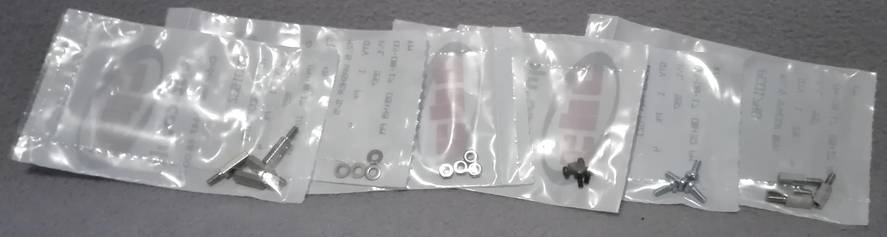
\includegraphics[width=0.9\linewidth]{photos/screws1.png}
    \caption*{Śrubki do zastosowań wewnątrz modelu}
\end{figure}
\begin{figure}[H]
    \centering
    \begin{subfigure}{0.32\textwidth}
        \centering
        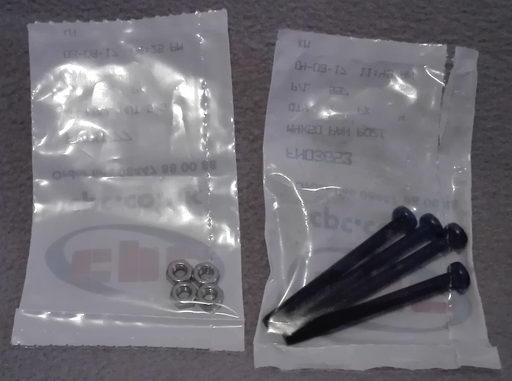
\includegraphics[width=0.9\linewidth]{photos/screws2.png}
        \caption*{Większe śruby do montażu mechanicznego}
    \end{subfigure}
    \begin{subfigure}{0.32\textwidth}
        \centering
        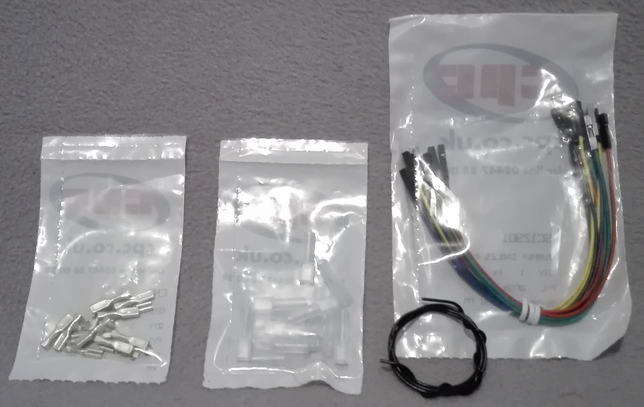
\includegraphics[width=0.9\linewidth]{photos/cables.png}
        \caption*{Zestaw kabli, złącz i gumowych osłon}
    \end{subfigure}
    \begin{subfigure}{0.32\textwidth}
        \centering
        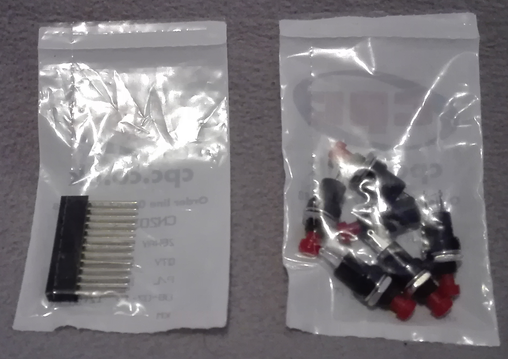
\includegraphics[width=0.9\linewidth]{photos/buttons.png}
        \caption*{Podwyższające złącze szpilkowe i przyciski}
    \end{subfigure}
\end{figure}

\section{Drukowanie}\label{sec:cover_printing}

Skorzystaliśmy z drukarki 3D znajdującej się w budynku Katedry Informatyki Akademii Górniczo
Hutniczej (KI AGH), by wydrukować elementy obudowy. Dostarczone w formacie stl schematy
przekonwertowaliśmy na format gcode rozumiany przez drukarkę.

\begin{figure}[H]
    \centering
    \begin{subfigure}{0.24\textwidth}
        \centering
        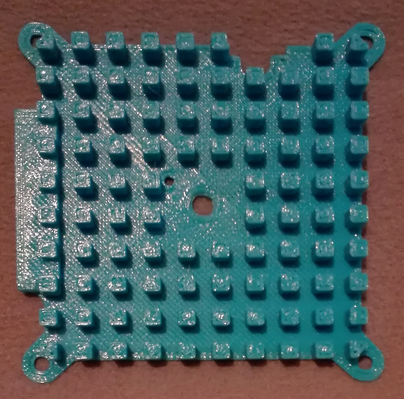
\includegraphics[width=0.9\linewidth]{photos/part1.png}
        \caption*{Radiator}
    \end{subfigure}
    \begin{subfigure}{0.24\textwidth}
        \centering
        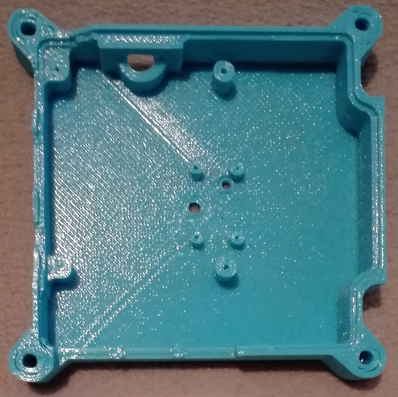
\includegraphics[width=0.9\linewidth]{photos/part2.png}
        \caption*{Podstawa}
    \end{subfigure}
    \begin{subfigure}{0.24\textwidth}
        \centering
        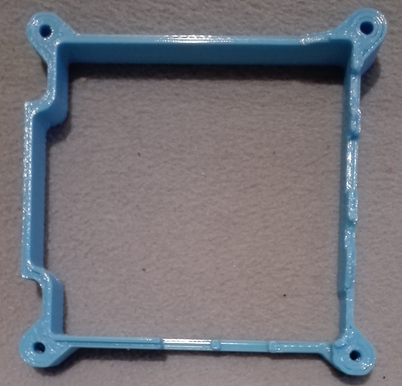
\includegraphics[width=0.9\linewidth]{photos/part3.png}
        \caption*{Środek}
    \end{subfigure}
    \begin{subfigure}{0.24\textwidth}
        \centering
        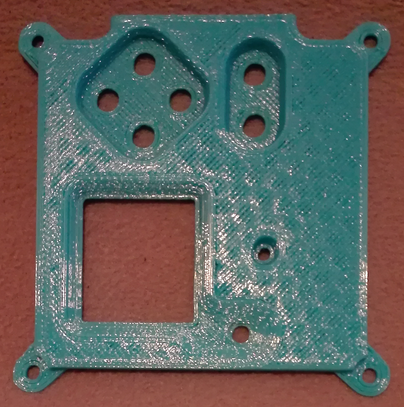
\includegraphics[width=0.9\linewidth]{photos/part4.png}
        \caption*{Panel główny}
    \end{subfigure}
\end{figure}

Każdy ze schematów dostarczony był w dwóch wersjach: normalnej i specjalnej na drukarki
gorszej jakości, które nierównomiernie ostygają. Asekuracyjnie wybraliśmy wersję drugą,
co okazało się błędem, ponieważ drukarka w budynku KI ostyga równomiernie i elementy
dodatkowe które miały w założeniu pomóc stygnąć, a później zostać oderwane, skleiły
się na stałe z modelem. Modelu tego ostatecznie nie wykorzystaliśmy przed błąd drukarki
który pojawił się pod koniec drukowania, a kolejne elementy drukowaliśmy już w wersji normalnej.

W trakcie drukowania natrafiliśmy na kilka problemów:
\begin{itemize}
    \item niezidentyfikowany błąd zatrzymał drukarkę w trakcie drukowania, a gorąca głowica
    stopiła jedną z nóżek drukowanego radiatora
    \item podczas drukowania ścianek bocznych ustawiliśmy zbyt małą prędkość drukowania,
    przez co ścianki drukowały się zbyt dokładnie i warstwy się nie połączyły, a ścianka
    rozwarstwiła
    \item uszkodzony fragment filamentu zaciął drukarkę, którą częściowo musieliśmy rozebrać,
    aby wyjąć uszkodzony fragment
\end{itemize}

W poradnikach drukowania znaleźliśmy informacje, że im mniejsza prędkość drukowania tym lepiej,
bo modele wychodzą dokładniejsze. Eksperymentalnie nauczyliśmy się, że dokładniejsze modele wcale
nie muszą być lepsze. Przez zbyt dokładne drukowanie ścianek zamiast jednej solidnej ścianki otrzymaliśmy
pięć pojedyńczych warstw zbudowanych jedna obok drugiej, które przez brak połączenia były bardzo kruche.

Mimo wszystkich przeciwności ostatecznie wydrukowaliśmy wszystkie elementy i zbudowaliśmy obudowę dla
mikrokomputera Raspberry.

\begin{figure}[H]
    \centering
    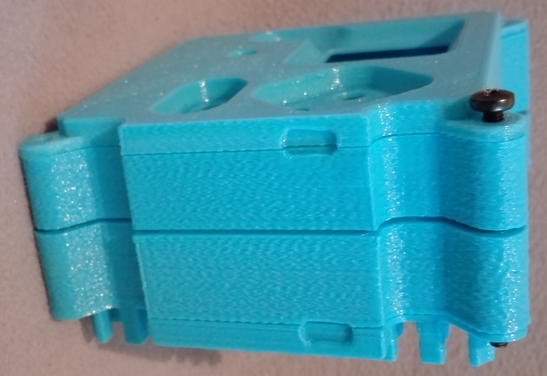
\includegraphics[width=0.6\linewidth]{photos/all.png}
\end{figure}


    \chapter{Porównanie wydajności Raspberry Pi 3, Raspberry Pi 1 oraz komputera klasy PC}\label{ch:performance}
    \section{Opis problemu}\label{sec:performance_introduction}

Naszym pierwszym zamierzeniem było dokonywanie na pokładzie stacji zarówno pomiarów
(wykonania zdjęć), jak również ich analizy (przy pomocy algorytmów uczenia maszynowego). Jednak już po
rozpoczęciu przygotowywania programu dowiedzieliśmy się o przeciwskazaniach do takiego
podejścia do problemu.

Zostaliśmy poinformowani, że na pokładzie ISS nie znajduje RaspberryPi 3
Model B, jak początkowo sądziliśmy, a znacznie wolniejszy Raspberry Pi 1 Model B+. W związku
z takim obrotem spraw postanowiliśmy dokonać pomiarów prędkości tych dwóch modeli, jak
również komputera stacjonarnego PC, w celu sprawdzenia, czy analiza zdjęć na pokładzie będzie
wydajnościowo możliwa.

ESA udostępniła zbiór zdjęć wykonanych przez Raspberry w poprzedniej edycji eksperymentu, jednak
wśród nich nie znajdowały się zdjęcia wykonane po ciemnej stronie globu. Było to kolejne przeciwskazanie
do pierwotnego pomysłu, ponieważ musielibysmy spreparować dane testowe wykorzystując zdjecia znalezione
w Internecie i wykonane przez inne urządzenia.

Nie mieliśmy wpływu na drugi problem, ale mogliśmy sprawdzić jak poważnym przeciwskazaniem jest pierwszy.
Postanowiliśmy zbadać wydajność modelu RaspberryPi 1 B+ i porównać ją z wydajnością modelu Raspberry 3 B oraz
komputerem stacjonarnym. Jako algorytm testowy postanowiliśmy wykorzystać metodę regresji logistycznej
wytrenowaną na zbiorze danych MNIST, ponieważ dane te są dostępne za darmo, a danych właściwe dla naszego
eksperymentu wykonamy dopiero w kolejnej jego fazie. Poniżej przedstawiamy wyniki czasowe ogólne jednego
przebiegu programu, oraz rozbite na zrobienie zdjęcia oraz jego analizę.

Próbą testową, którą kamera rejestrowała był zawsze obraz cyfry 8. Niestety prosty model liniowy jakim jest
regresja logistyczna w obrazie cyfry 8 rozpoznawał wszystkie możliwe cyfry. W naszym przypadku nie był to
jednak problem, ponieważ nie liczyła się dla nas poprawność rozpoznania, a jedynie czas przeprowadzenia analizy.

\section{Wyniki}\label{sec:performance_results}

\begin{table}[H]
    \centering
    \begin{threeparttable}
        \caption{Komputer klasy PC}
        \begin{tabular}{|l|l|ccc|}
            \toprule
            \thead{Rozpoznana \\ cyfra} & & \thead{Zrobienie \\ zdjęcia} &
            \thead{Analiza \\ zdjęcia} & \thead{Pojedyńczy \\ przebieg} \\
            \midrule
            1 & Najkrótszy czas[s] & 0.000 & 0.006 & 0.010 \\
            & Średni czas[s] & 0.000 & 0.006 & 0.010 \\
            & Najdłuższy czas[s] & 0.001 & 0.016 & 0.020 \\
            \midrule
            7 & Najkrótszy czas[s] & 0.000 & 0.006 & 0.010 \\
            & Średni czas[s] & 0.000 & 0.007 & 0.011 \\
            & Najdłuższy czas[s] & 0.001 & 0.012 & 0.016 \\
            \midrule
            8 & Najkrótszy czas[s] & 0.000 & 0.006 & 0.010 \\
            & Średni czas[s] & 0.000 & 0.006 & 0.010 \\
            & Najdłuższy czas[s] & 0.001 & 0.007 & 0.012 \\
            \midrule
            6 & Najkrótszy czas[s] & 0.000 & 0.006 & 0.010 \\
            & Średni czas[s] & 0.000 & 0.006 & 0.010 \\
            & Najdłuższy czas[s] & 0.001 & 0.007 & 0.011 \\
            \bottomrule
        \end{tabular}
        \begin{tablenotes}
            \item Procesor IntelCore i7-4790 3.60 Ghz
            \item RAM 16 GB
        \end{tablenotes}
    \end{threeparttable}
\end{table}

\begin{table}[H]
    \centering
    \begin{threeparttable}
        \caption{Raspberry Pi 1 Model B+}
        \begin{tabular}{|l|l|ccc|}
            \toprule
            \thead{Rozpoznana \\ cyfra} & & \thead{Zrobienie \\ zdjęcia} &
            \thead{Analiza \\ zdjęcia} & \thead{Pojedyńczy \\ przebieg} \\
            \midrule
            0 & Najkrótszy czas[s] & 0.106 & 0.739 & 0.933 \\
            & Średni czas[s] & 1.038 & 0.746 & 1.875 \\
            & Najdłuższy czas[s] & 2.385 & 0.760 & 2.097 \\
            \midrule
            2 & Najkrótszy czas[s] & 0.105 & 0.741 & 0.920 \\
            & Średni czas[s] & 0.881 & 0.765 & 1.769 \\
            & Najdłuższy czas[s] & 4.503 & 0.849 & 5.334 \\
            \midrule
            4 & Najkrótszy czas[s] & 0.104 & 0.737 & 0.936 \\
            & Średni czas[s] & 0.563 & 0.746 & 1.454 \\
            & Najdłuższy czas[s] & 1.557 & 0.759 & 2.373 \\
            \midrule
            7 & Najkrótszy czas[s] & 0.102 & 0.740 & 0.920 \\
            & Średni czas[s] & 0.554 & 0.751 & 1.421 \\
            & Najdłuższy czas[s] & 2.313 & 0.763 & 3.135 \\
            \midrule
            8 & Najkrótszy czas[s] & 0.174 & 0.743 & 0.958 \\
            & Średni czas[s] & 0.505 & 0.754 & 1.562 \\
            & Najdłuższy czas[s] & 2.720 & 0.763 & 3.538 \\
            \bottomrule
        \end{tabular}
        \begin{tablenotes}
            \item Procesor Broadcom CoS BCM2835 700 Mhz
            \item RAM: 512 MB
        \end{tablenotes}
    \end{threeparttable}
\end{table}

\begin{table}[H]
    \centering
    \begin{threeparttable}
        \caption{Raspberry Pi 3 Model B}
        \begin{tabular}{|l|l|ccc|}
            \toprule
            \thead{Rozpoznana \\ cyfra} & & \thead{Zrobienie \\ zdjęcia} &
            \thead{Analiza \\ zdjęcia} & \thead{Pojedyńczy \\ przebieg} \\
            \midrule
            0 & Najkrótszy czas[s] & 0.014 & 0.073 & 0.106 \\
            & Średni czas[s] & 0.014 & 0.133 & 0.177 \\
            & Najdłuższy czas[s] & 0.015 & 0.144 & 0.191 \\
            \midrule
            9 & Najkrótszy czas[s] & 0.007 & 0.080 & 0.104 \\
            & Średni czas[s] & 0.014 & 0.132 & 0.177 \\
            & Najdłuższy czas[s] & 0.015 & 0.135 & 0.180 \\
            \midrule
            1 & Najkrótszy czas[s] & 0.007 & 0.072 & 0.097 \\
            & Średni czas[s] & 0.014 & 0.132 & 0.177 \\
            & Najdłuższy czas[s] & 0.025 & 0.186 & 0.230 \\
            \midrule
            3 & Najkrótszy czas[s] & 0.014 & 0.124 & 0.168 \\
            & Średni czas[s] & 0.014 & 0.132 & 0.177 \\
            & Najdłuższy czas[s] & 0.014 & 0.135 & 0.179 \\
            \midrule
            7 & Najkrótszy czas[s] & 0.014 & 0.080 & 0.125 \\
            & Średni czas[s] & 0.014 & 0.134 & 0.179 \\
            & Najdłuższy czas[s] & 0.025 & 0.148 & 0.217 \\
            \midrule
            4 & Najkrótszy czas[s] & 0.014 & 0.131 & 0.176 \\
            & Średni czas[s] & 0.014 & 0.132 & 0.176 \\
            & Najdłuższy czas[s] & 0.014 & 0.132 & 0.176 \\
            \midrule
            5 & Najkrótszy czas[s] & 0.015 & 0.069 & 0.104 \\
            & Średni czas[s] & 0.015 & 0.138 & 0.183 \\
            & Najdłuższy czas[s] & 0.023 & 0.141 & 0.195 \\
            \midrule
            6 & Najkrótszy czas[s] & 0.007 & 0.068 & 0.092 \\
            & Średni czas[s] & 0.012 & 0.216 & 0.251 \\
            & Najdłuższy czas[s] & 0.034 & 0.335 & 0.426 \\
            \midrule
            8 & Najkrótszy czas[s] & 0.007 & 0.072 & 0.097 \\
            & Średni czas[s] & 0.014 & 0.139 & 0.192 \\
            & Najdłuższy czas[s] & 0.015 & 0.146 & 0.194 \\
            \midrule
            2 & Najkrótszy czas[s] & 0.007 & 0.072 & 0.097 \\
            & Średni czas[s] & 0.016 & 0.163 & 0.227 \\
            & Najdłuższy czas[s] & 0.028 & 0.267 & 0.356 \\
            \bottomrule
        \end{tabular}
        \begin{tablenotes}
            \item CPU: 4x ARM Cortex-A53, 1.2GHz (Quad Core 1.2GHz Broadcom BCM2837 64bit CPU)
            \item RAM: 1GB LPDDR2 (900 MHz)
            \item Rozbieżności w przypadku 6 i 2 były bardzo duże, najpierw seria bardzo szybkich rozpoznań,
            później seria bardzo powolnych.
        \end{tablenotes}
    \end{threeparttable}
\end{table}

\section{Opracowanie wyników}\label{sec:performance_results_preparation}

\begin{table}[H]
    \centering
    \begin{threeparttable}
        \caption{Uśredniony czas wszystkich prób}
        \begin{tabular}{|lccc|}
            \toprule
            & Zrobienie zdjęcia & Analiza zdjęcia & Pojedyńczy przebieg \\
            \midrule
            RaspberryPi 1 & 0.708 & 0.752 & 1.616 \\
            RaspberryPi 3 & 0.014 & 0.132 & 0.176 \\
            PC & 0.000 & 0.006 & 0.010 \\
            \bottomrule
        \end{tabular}
    \end{threeparttable}
\end{table}

\begin{table}[H]
    \centering
    \begin{threeparttable}
        \caption{Ilorazy poszczególnych wyników}
        \begin{tabular}{|lccc|}
            \toprule
            & Zrobienie zdjęcia & Analiza zdjęcia & Pojedyńczy przebieg \\
            \midrule
            Iloraz Pi1/Pi3 & 50,5x & 5,5x & 9x \\
            Iloraz Pi3/PC & 14x & 22x & 17,5x \\
            Iloraz Pi1/PC & 708x & 125x & 161,5x \\
            \bottomrule
        \end{tabular}
    \end{threeparttable}
\end{table}

\large Dodatkowe zastrzeżenia odnośnie Raspberry Pi 1: \normalsize
\begin{itemize}
    \item bardzo wolne łącze ethernetowe
    \footnotesize (poczta Gmail otwierała się ok 2 min, dla porównania przy dokładnie
    tej samej konfiguracji pozostałego sprzętu, jak również dokładnie tym samym egzemplarzem systemu, na
    Raspberry Pi 3 trwało to 0,5s) \normalsize \\
    \item niewydolność pozostałych interfejsów wejścia/wyjścia
    \footnotesize (w trakcie robienia zdjęcia przy pomocy modułu kamery, obraz
    na ekranie podpiętym pod HDMI stawał się czarny i wracał dopiero gdy zdjęcie zostało zapisane przez
    program) \normalsize \\
\end{itemize}

\section{Wnioski}\label{sec:performance_conclusion}

Najprawdopodobniej wykonanie zdjęcia na Raspberry Pi 1 było tak mało wydajne z powodu
niewydolności interfejsów i mniejszej mocy obliczeniowej tego modelu.
Nie bez znaczenia jest też fakt, że model 1 posiada procesor jednordzeniowy, zaś model 3 - czterordzeniowy.
To wszystko tłumaczy 50x wolniejsze działanie w porównaniu z Raspberry Pi 3.

Analiza zdjęcia na wszystkich 3 obiektach testowych była najbardziej stała czasowo, a jako
że to był główny cel naszego eksperymentu, to te wyniki są dla nas najważniejsze. Raspberry Pi 1
jest średnio 5,5x wolniejsze na samej analizie zdjęcia, które w tym przypadku było wykonywane
metodą prostej regresji liniowej.
W przypadku bardziej złożonych obliczeniowo modeli uczenia maszynowego można spodziewać się, że
rozbieżności czasowe będą dużo bardziej widoczne, dlatego musimy zrezygnować z analizy zdjęć
na stacji kosmicznej przez niską moc obliczeniową sprzętu.

Analizy zdjęć dokonamy na komputerze PC, już po wykonaniu części eksperymentu mającej
miejsce na pokładzie ISS.

Zmiana założeń eksperymentu niosła za sobą, poza rozwiązaniem problemu z wydajnością, także negatywne
konsekwencje. Miejsce na karcie pamięci mikrokomputera na stacji ISS które może zająć każdy zespół jest
ograniczone, dlatego też w kolejnej części eksperymentu próbowaliśmy znaleźć sposób na redukcję rozmiaru
wykonanych zdjęć.


    \chapter{Kompresja zdjęć metodą redukcji kolorów}
    \section{Zarys problemu}

Po przeanalizowaniu wydajności Raspberry Pi, postanowiliśmy zredukować zakres odpowiedzialności płytki, aby będąc w kosmosie robiła zdjęcia powierzchni Ziemi i zapisywała je na karcie pamięci.
Zdjęcia mają następnie trafić do nas, w celu dalszej analizy.
Zależy nam na dużej ilości danych, ale ponieważ zasady konkursu (oraz, rzecz jasna, pojemność karty pamięci płytki Raspberry Pi) narzucają na nas ograniczenia względem zurzytej przestrzeni dyskowej,
chcemy przechowywać zdjęcia o jak najmniejszym rozmiarze.

Najpowszechniej używane dziś formaty zapisu plików z obrazami to .jpg oraz .png. Format .png zapewnia bezstratną kompresję obrazu. Format .jpg kompresuje stratnie, choć straty te nie są doskonale widoczne gołym okiem i sprawiają problem przede wszystkim gdy zależy nam na zachowaniu bardzo wysokiej rozdzielczości zdjęcia. W zamian .jpg oferuje znacznie mniejszy niż .png rozmiar pliku.

Ponieważ zamierzamy analizować zdjęcia Ziemi nocą, stać nas na założenie, że zdjęcia te będą miały duży kontrast - ciemne i jasne połacie terenu. Stąd też akceptowalnym sposobem kompresji zdjęcia jest redukcja jego kolorów.

W niniejszym sprawozdaniu prezentujemy nasze wyniki badania wpływu redukcji kolorów obrazu różnymi sposobami na jego rozmiar.

\section{Algorytm k-means}

Algorytm k-means jest dzieli dane punkty na $k$ klastrów punktów najbardziej podobnych, co w przypadku obrazów jest równoważne
znalezieniu $k$ kolorów najbardziej reprezentatywnych dla obrazu.

O samym algorytmie przeczytać można więcej na poniższej stronie internetowej: \url{https://www.datascience.com/blog/k-means-clustering}

\subsection{Zastosowanie algorytmu w kompresji obrazów}
K-means można zaaplikować do obrazów następująco:

\begin{enumerate}
\item Za pomocą algorytmu znaleźć $k$ kolorów najbardziej "reprezentatywnych" dla obrazu
\item Każdy piksel w obrazie zmapować na kolor reprezentatywny najbliższy do koloru tegoż piksela
\item Obraz z ograniczoną do $k$ liczbą kolorów potrzebuje mniej bitów, by dany kolor zakodować, dzięki czemu może zajmować mniej pamięci.
\end{enumerate}

\section{Faktyczna redukcja rozmiaru pliku poprzez redukcję długości kodowania kolorów}

Oczywiście samo zmniejszenie liczby kolorów obrazu nie wystarczy, aby miał on mniejszy rozmiar - trzeba jeszcze zmodyfikować głębię koloru obrazu, by plik go zawierający korzystał z informacji o tym górnym ograniczeniu i mógł sobie pozwolić na kodowanie kolorów mniejszą liczbą bitów.
W systemie operacyjnym Linux (a w szczególności systemie Raspbian) istnieją narzędzia \textbf{pngtopnm}, \textbf{pnmquant} oraz \textbf{pnmtopng}, których kombinacja pozwala na osiągnięcie tego celu.

W szczególności efekt ten daje następujące wywołanie w terminalu:

\begin{lstlisting}
> pngtopnm input.png | pnmquant $NUM_COLORS | pnmtopng output.png
\end{lstlisting}

Dla zdjęcia posiadającego większą liczbę kolorów niż podana, narzędzie to znajduje sobie znanym sposobem odpowiednią liczbę reprezentatywnych kolorów. Nie dzieje się tak, gdy narzędzie stwierdzi, że obraz ma już odpowiednio niską liczbę kolorów. Zatem uprzednia redukcja kolorów nie jest konieczna.

\section{Pomiary}

Pomiary faktycznego wpływu redukcji kolorów na rozmiar pliku wykonano na 300 zdjęciach kotów zawartych w zbiorze: \url{https://www.kaggle.com/c/dogs-vs-cats/data}

Zapisano i zmierzono rozmiary wszystkich tych zdjęć po różnych przekształceniach:

\begin{itemize}
\item oryginalne zdjęcie w formacie .jpg
\item oryginalne zdjęcie w formacie .png
\item dla liczby kolorów do których chcemy zredukować $K \in [1, 2, 4, 8, 16, 32]$
	\begin{itemize}
      \item zdjęcie z kolorami zredukowanymi do $K$  i odpowiednio zredukowaną głębią kolorów w formacie .png przez ww. narzędzia systemowe
      \item dla liczby iteracji algorytmu k-means $I \in [1, 2, 4, 8, 16, 32]$ zdjęcie z kolorami zredukowanymi do $K$ przez k-means w $I$ iteracjach
      \begin{itemize}
        \item zapisane w formacie .jpg
        \item zapisane w formacie .png
        \item zapisane w formacie .png z głębią kolorów zredukowaną przez ww. narzędzia systemowe
      \end{itemize}
	\end{itemize}
\end{itemize}

Warto dodać, że narzędzie systemowe nie pozwala operować na plikach .jpg.

\subsection{Wyniki pomiarów}

W poniższej tabeli zobaczyć można zagregowane średnie rozmiary (w bajtach) zdjęć poddanych różnym przeróbkom.

Oznaczenia:
\begin{itemize}
	\item $num\_centroids$ - liczba kolorów, do których zredukowano obraz. Jeżeli $num\_centroids = 0$, obraz w tym wypadku nie miał redukowanych kolorów przez k-means.
    \item $num\_iterations$ - liczba iteracji algorytmu k-means. Jeżeli $num\_centroids \neq 0$ oraz $num\_iterations = 0$ oznacza to obraz przepuszczony przez narzędzie do redukcji głębi bez uprzedniej redukcji kolorów algorytmem k-means.
    \item $new\_format$ - format zapisu obrazu. $jpg$ i $png$ oznaczają zapis obrazu w tych formatach bez przepuszczania go przez narzędzie redukujące głębię kolorów pliku. $red.png$ oznacza plik .png przepuszczony przez to narzędzie.
\end{itemize}

\begin{figure}[H]
	\begin{tabular}{llrrr}
\toprule
   & \{\} & \multicolumn{3}{l}{new\_size} \\
   & \{\} & \multicolumn{3}{l}{mean} \\
   & new\_format &           jpg &            png &       red.png \\
num\_centroids & num\_iterations &               &                &               \\
\midrule
0  & 0  &  22591.833887 &  190394.697674 &           -- \\
1  &    &           -- &            -- &   4138.551495 \\
   & 1  &   3078.192691 &    1232.382060 &    113.192691 \\
   & 2  &   3078.192691 &    1232.382060 &    113.192691 \\
   & 4  &   3078.192691 &    1232.382060 &    113.192691 \\
   & 8  &   3078.192691 &    1232.382060 &    113.192691 \\
   & 16 &   3078.192691 &    1232.382060 &    113.192691 \\
   & 32 &   3078.192691 &    1232.382060 &    113.192691 \\
2  & 0  &           -- &            -- &   4138.551495 \\
   & 1  &  13131.441860 &    5999.295681 &   2821.644518 \\
   & 2  &  15391.006645 &    6949.458472 &   3356.534884 \\
   & 4  &  15592.777409 &    7050.714286 &   3419.784053 \\
   & 8  &  15673.312292 &    7004.877076 &   3402.322259 \\
   & 16 &  15878.810631 &    7138.245847 &   3474.372093 \\
   & 32 &  16052.049834 &    7176.561462 &   3504.578073 \\
4  & 0  &           -- &            -- &  10102.186047 \\
   & 1  &  17658.332226 &   10087.471761 &   5428.601329 \\
   & 2  &  21845.857143 &   16130.176080 &   8795.946844 \\
   & 4  &  22943.073090 &   17221.139535 &   9508.086379 \\
   & 8  &  23252.893688 &   17251.604651 &   9582.458472 \\
   & 16 &  23183.923588 &   17159.205980 &   9536.169435 \\
   & 32 &  23112.166113 &   17090.591362 &   9489.687708 \\
8  & 0  &           -- &            -- &  17909.166113 \\
   & 1  &  20786.089701 &   15370.013289 &   8804.810631 \\
   & 2  &  23156.066445 &   23918.139535 &  13427.544850 \\
   & 4  &  23462.485050 &   30719.262458 &  16648.903654 \\
   & 8  &  23887.847176 &   32072.269103 &  17638.451827 \\
   & 16 &  24175.661130 &   31750.548173 &  17714.531561 \\
   & 32 &  24167.664452 &   31708.186047 &  17762.408638 \\
16 & 0  &           -- &            -- &  26527.903654 \\
   & 1  &  22730.674419 &   21430.302326 &  12068.126246 \\
   & 2  &  23624.299003 &   32003.784053 &  17148.601329 \\
   & 4  &  23558.963455 &   40450.272425 &  20581.302326 \\
   & 8  &  23636.418605 &   48979.063123 &  24087.428571 \\
   & 16 &  23670.710963 &   52313.169435 &  26012.232558 \\
   & 32 &  23716.657807 &   52680.511628 &  26652.936877 \\
32 & 0  &           -- &            -- &  37409.435216 \\
   & 1  &  23809.674419 &   28604.551495 &  15666.920266 \\
   & 2  &  23771.159468 &   40778.249169 &  21146.179402 \\
   & 4  &  23602.438538 &   50020.584718 &  25060.913621 \\
   & 8  &  23563.033223 &   57867.332226 &  28458.651163 \\
   & 16 &  23415.744186 &   69236.189369 &  32988.189369 \\
   & 32 &  23349.152824 &   77122.053156 &  36404.614618 \\
\bottomrule
\end{tabular}

\end{figure}

\subsection{Porównanie sposobów kompresji}

\subsubsection{Porównanie formatów .jpg z redukcją kolorów algorytmem k-means i z zachowaniem oryginalnych kolorów}
\label{m:jpg_vs_jpg}
Poniższa tabela prezentuje średni stosunek wielkości plików .jpg (z redukcją kolorów algorytmem k-means) do oryginalnego zdjęcia jako .jpg:
\begin{figure}[H]
	\begin{tabular}{lrrrrrrr}
\toprule
num\_iterations &   0  &        1  &        2  &        4  &        8  &        16 &        32 \\
num\_centroids &      &           &           &           &           &           &           \\
\midrule
0             &  1.0 &       -- &       -- &       -- &       -- &       -- &       -- \\
1             &  -- &  0.136252 &  0.136252 &  0.136252 &  0.136252 &  0.136252 &  0.136252 \\
2             &  -- &  0.581247 &  0.681264 &  0.690195 &  0.693760 &  0.702856 &  0.710524 \\
4             &  -- &  0.781625 &  0.966980 &  1.015547 &  1.029261 &  1.026208 &  1.023032 \\
8             &  -- &  0.920071 &  1.024975 &  1.038538 &  1.057366 &  1.070106 &  1.069752 \\
16            &  -- &  1.006146 &  1.045701 &  1.042809 &  1.046237 &  1.047755 &  1.049789 \\
32            &  -- &  1.053906 &  1.052201 &  1.044733 &  1.042989 &  1.036469 &  1.033522 \\
\bottomrule
\end{tabular}

\end{figure}

Wnioski: \ref{f:jpg_vs_jpg}

\subsubsection{Porównanie formatów .jpg i .png}
\label{m:png_vs_jpg}

Poniższa tabela prezentuje średni stosunek wielkości plików .png (bez redukcji głębi kolorów narzędziami systemowymi) do odpowiadających im przekształceniami plików .jpg:
\begin{figure}[H]
	\begin{tabular}{lrrrrrrr}
\toprule
num\_iterations &        0  &        1  &        2  &        4  &        8  &        16 &        32 \\
num\_centroids &           &           &           &           &           &           &           \\
\midrule
0             &  8.427589 &       -- &       -- &       -- &       -- &       -- &       -- \\
1             &       -- &  0.400359 &  0.400359 &  0.400359 &  0.400359 &  0.400359 &  0.400359 \\
2             &       -- &  0.456865 &  0.451527 &  0.452178 &  0.446930 &  0.449545 &  0.447081 \\
4             &       -- &  0.571258 &  0.738363 &  0.750603 &  0.741912 &  0.740134 &  0.739463 \\
8             &       -- &  0.739437 &  1.032910 &  1.309293 &  1.342619 &  1.313327 &  1.312009 \\
16            &       -- &  0.942792 &  1.354698 &  1.716980 &  2.072186 &  2.210038 &  2.221245 \\
32            &       -- &  1.201384 &  1.715451 &  2.119297 &  2.455852 &  2.956822 &  3.302991 \\
\bottomrule
\end{tabular}

\end{figure}

Wnioski: \ref{f:png_vs_jpg}


\subsubsection{Porównanie formatu .png z redukcją głębi i bez}

\label{m:red_vs_png}
Poniższa tabela prezentuje średni stosunek wielkości plików .png z redukcją głębi kolorów narzędziami systemowymi (i doborem kolorów za pomocą algorytmu k-means) do odpowiadających im przekształceniami plików .png bez redukcji:
\begin{figure}[H]
	\begin{tabular}{lrrrrrrr}
\toprule
num\_iterations &  0  &        1  &        2  &        4  &        8  &        16 &        32 \\
num\_centroids &     &           &           &           &           &           &           \\
\midrule
0             & -- &       -- &       -- &       -- &       -- &       -- &       -- \\
1             & -- &  0.091849 &  0.091849 &  0.091849 &  0.091849 &  0.091849 &  0.091849 \\
2             & -- &  0.470329 &  0.482992 &  0.485027 &  0.485708 &  0.486726 &  0.488337 \\
4             & -- &  0.538153 &  0.545310 &  0.552117 &  0.555453 &  0.555747 &  0.555258 \\
8             & -- &  0.572856 &  0.561396 &  0.541970 &  0.549960 &  0.557928 &  0.560184 \\
16            & -- &  0.563134 &  0.535830 &  0.508805 &  0.491790 &  0.497241 &  0.505935 \\
32            & -- &  0.547707 &  0.518565 &  0.501012 &  0.491791 &  0.476459 &  0.472039 \\
\bottomrule
\end{tabular}

\end{figure}

Wnioski: \ref{f:red_vs_png}

\subsubsection{Porównanie rozmiaru doboru kolorów algorytmem k-means i systemowym w zdjęciach zdjęć w formacie .png z redukcją głębi kolorów}

\label{m:red_vs_red}

Poniższa tabela prezentuje średni stosunek wielkości plików .png, gdzie uprzednio zastosowano redukcję kolorów algorytmem k-means do plików .png z redukcją głębi kolorów narzędziami systemowymi:

\begin{figure}[H]
	\begin{tabular}{lrrrrrrr}
\toprule
num\_iterations &   0  &        1  &        2  &        4  &        8  &        16 &        32 \\
num\_centroids &      &           &           &           &           &           &           \\
\midrule
0             &  -- &       -- &       -- &       -- &       -- &       -- &       -- \\
1             &  1.0 &  0.027351 &  0.027351 &  0.027351 &  0.027351 &  0.027351 &  0.027351 \\
2             &  1.0 &  0.681795 &  0.811041 &  0.826324 &  0.822105 &  0.839514 &  0.846813 \\
4             &  1.0 &  0.537369 &  0.870697 &  0.941191 &  0.948553 &  0.943971 &  0.939370 \\
8             &  1.0 &  0.491637 &  0.749758 &  0.929630 &  0.984884 &  0.989132 &  0.991805 \\
16            &  1.0 &  0.454922 &  0.646436 &  0.775836 &  0.908003 &  0.980561 &  1.004713 \\
32            &  1.0 &  0.418796 &  0.565263 &  0.669909 &  0.760735 &  0.881815 &  0.973140 \\
\bottomrule
\end{tabular}

\end{figure}

Wnioski: \ref{f:red_vs_red}

\subsubsection{Porównanie obrazów w formacie .png ze zredukowaną głębią kolorów z oryginalnym zdjęciem w formacie .jpg}

\label{m:red_vs_jpg}

Poniższa tabela prezentuje średni stosunek wielkości plików .png, gdzie uprzednio zredukowano głębię kolorów narzędziami systemowymi (uprzednio redukując kolory algorytmem k-means tam, gdzie $num\_iterations > 0)$ do oryginalnego zdjęcia zapisanego w formacie .jpg:

\begin{figure}[H]
	\begin{tabular}{lrrrrrrr}
\toprule
num\_iterations &        0  &        1  &        2  &        4  &        8  &        16 &        32 \\
num\_centroids &           &           &           &           &           &           &           \\
\midrule
0             &       -- &       -- &       -- &       -- &       -- &       -- &       -- \\
1             &  0.183188 &  0.005010 &  0.005010 &  0.005010 &  0.005010 &  0.005010 &  0.005010 \\
2             &  0.183188 &  0.124897 &  0.148573 &  0.151373 &  0.150600 &  0.153789 &  0.155126 \\
4             &  0.447161 &  0.240290 &  0.389342 &  0.420864 &  0.424156 &  0.422107 &  0.420049 \\
8             &  0.792727 &  0.389734 &  0.594354 &  0.736943 &  0.780745 &  0.784112 &  0.786231 \\
16            &  1.174225 &  0.534181 &  0.759062 &  0.911006 &  1.066201 &  1.151400 &  1.179760 \\
32            &  1.655883 &  0.693477 &  0.936010 &  1.109291 &  1.259688 &  1.460182 &  1.611406 \\
\bottomrule
\end{tabular}

\end{figure}

Wnioski: \ref{f:red_vs_jpg}

\section{Wnioski}

\subsection{Interpretacja pomiarów}

\subsubsection{Porównanie formatów .jpg z redukcją kolorów algorytmem k-means i z zachowaniem oryginalnych kolorów}

\label{f:jpg_vs_jpg}

\begin{figure}[H]
	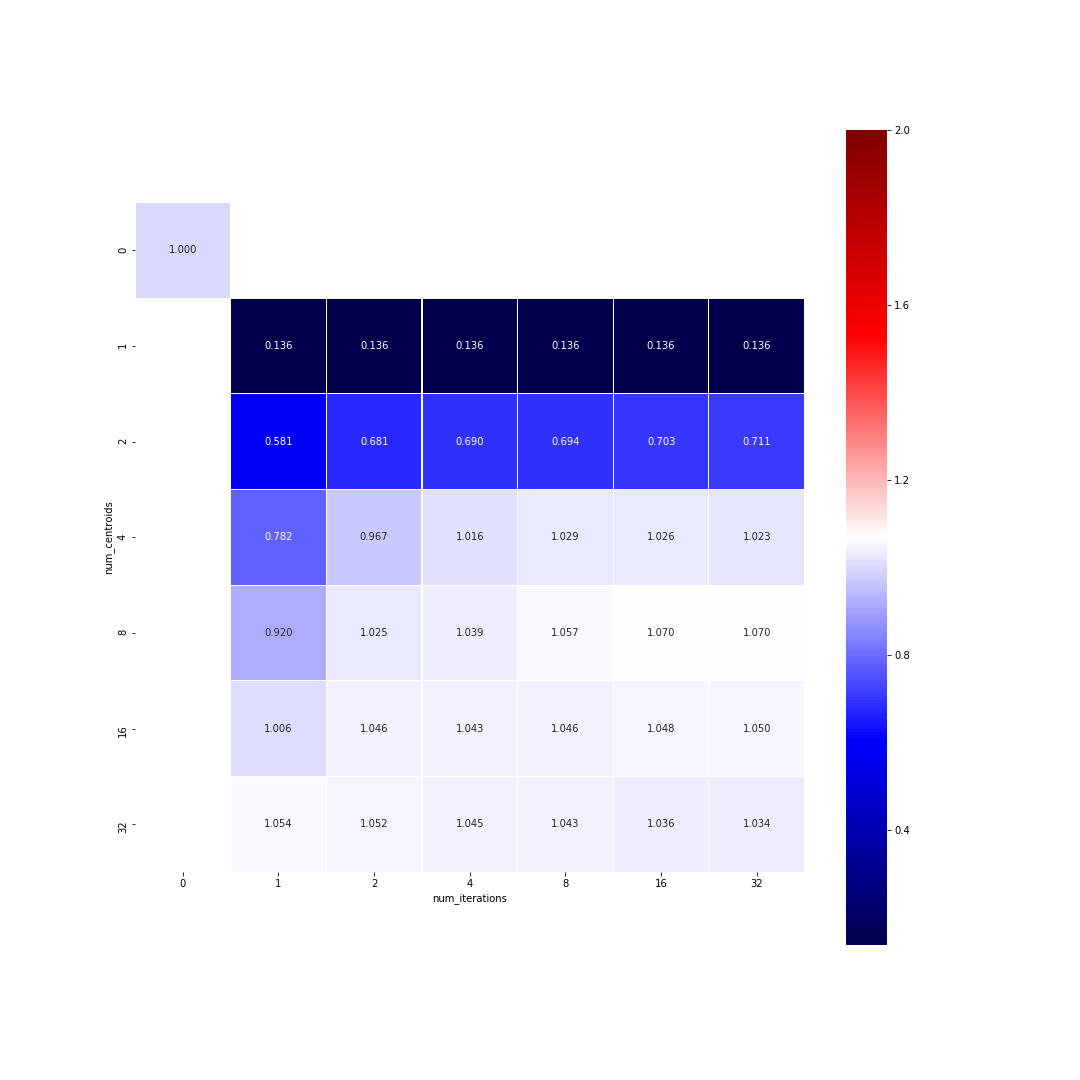
\includegraphics[width=0.9\textwidth]{photos/plots/jpg_vs_jpg}
    \caption{Wykres jakości wyników z tabeli \ref{m:jpg_vs_jpg}}
\end{figure}

Wprawdzie przy redukcji kolorów zdjęcia do jednego lub dwóch, daje to realną poprawę w porównaniu z rozmiarem oryginalnego zdjęcia. Widać jednak, że już przy czterech kolorach przestaje to powodować dużą różnicę w rozmiarze tak kompresowanych zdjęć.

\subsubsection{Porównanie formatów .jpg i .png}
\label{f:png_vs_jpg}

\begin{figure}[H]
	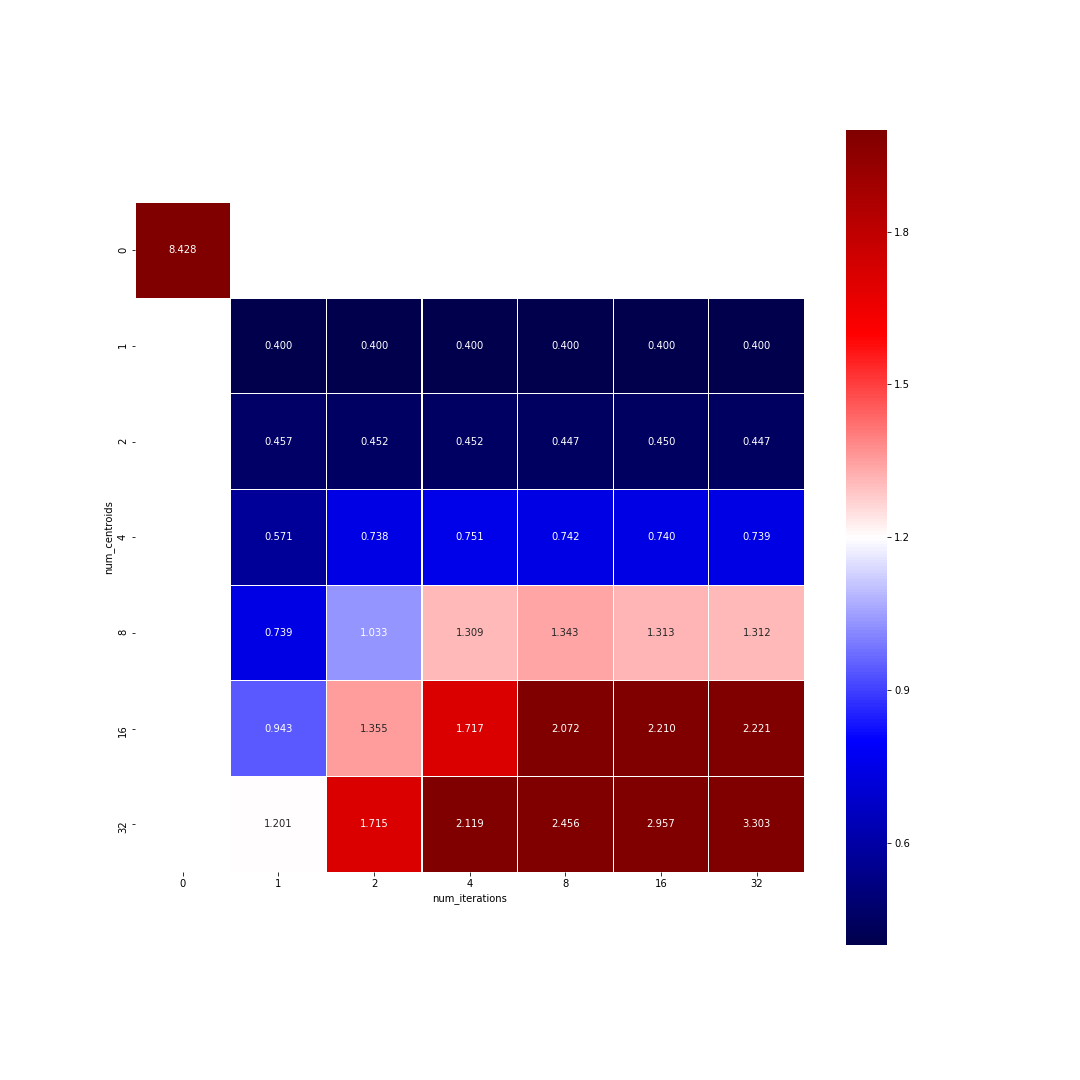
\includegraphics[width=0.9\textwidth]{photos/plots/png_vs_jpg}
    \caption{Wykres jakości wyników z tabeli \ref{m:png_vs_jpg}}
\end{figure}

Oryginalne zdjęcie zapisane w formacie .png jest ponad 8 razy większe niż to samo zdjęcie w formacie .jpg.
Choć sama redukcja kolorów obrazu (bez sprzętowej redukcji głębi obrazu) na początku działa na korzyść formatu .png. Jednak już przy redukcji do 8 kolorów widać, że na dłuższą metę nie jest ona wystarczająca, aby format .png dawał przewagę nad .jpg. Łącząc tę wiedzę z rezultatami z \ref{f:jpg_vs_jpg} można wysnuć wniosek, że ponieważ .png ze zredukowanymi kolorami nie daje przewagi nad .jpg z tak samo zredukowanymi kolorami, to nie będzie też dawać przewagi nad oryginalnym zdjęciem w formacie .jpg

\subsubsection{Porównanie formatu .png z redukcją głębi i bez}
\label{f:red_vs_png}

\begin{figure}[H]
	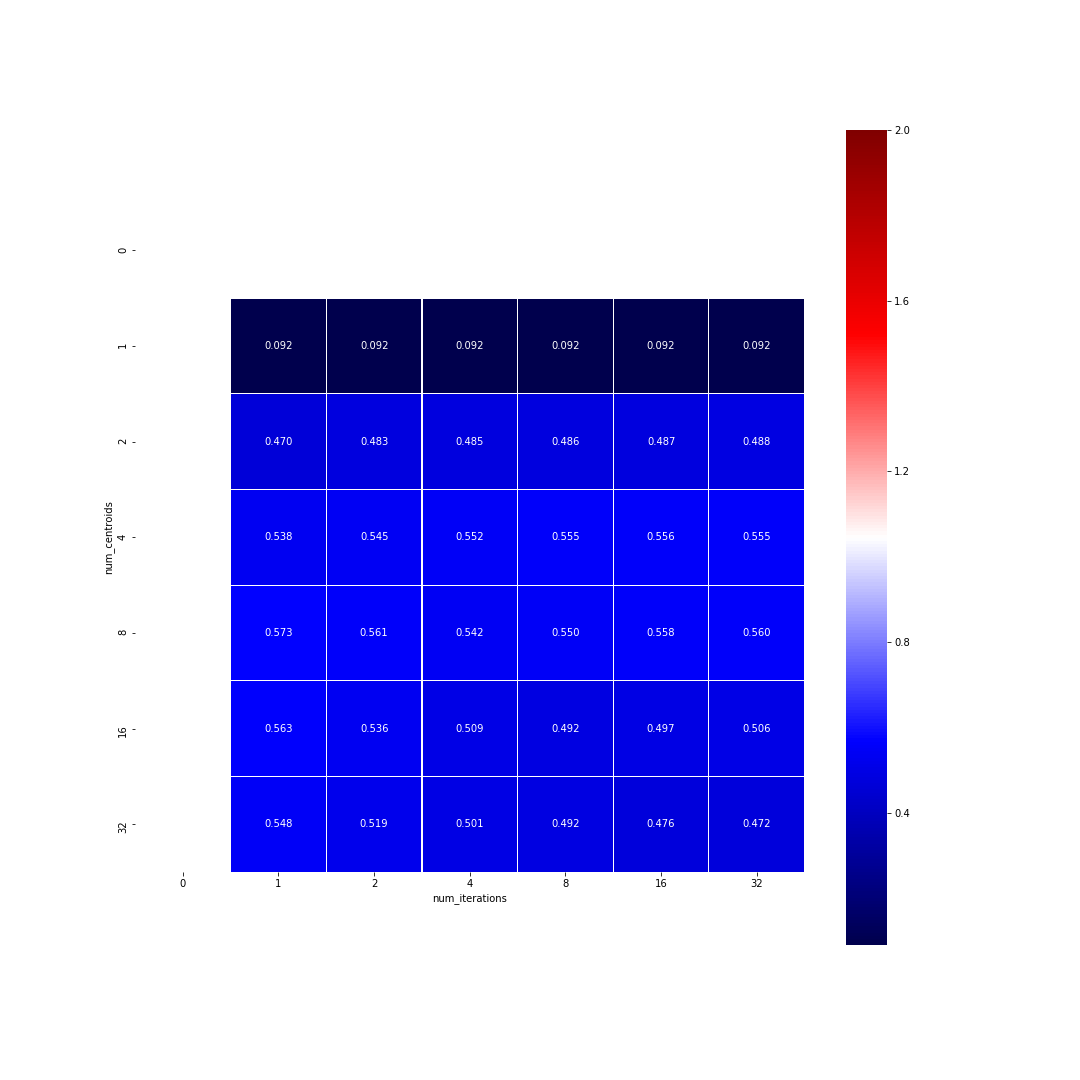
\includegraphics[width=0.9\textwidth]{photos/plots/red_vs_png}
    \caption{Wykres jakości wyników z tabeli \ref{m:red_vs_png}}
\end{figure}

Tutaj widać jednoznacznie, że użycie narzędzia systemowwego do redukcji głębi kolorów plików .png ze zdjęciami skutecznie obniża ich rozmiar ponad dwukrotnie. Co więcej, ponieważ oba zdjęcia mają uprzednio zredukowane kolory (za pomocą algorytmu k-means), redukcja głębi kolorów nie powoduje dalszych strat w jakości.

\begin{figure}[H]
  \centering
  \begin{minipage}[b]{0.4\textwidth}
    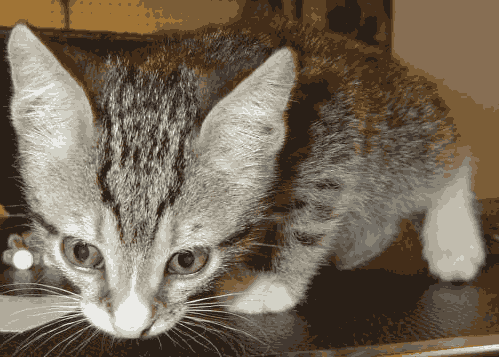
\includegraphics[width=\textwidth]{photos/kmeans_16_32}
    \caption{Zdjęcie zredukowane do 16 kolorów przed redukcją głębi kolorów pliku (91294 B)}
  \end{minipage}
  \hfill
  \begin{minipage}[b]{0.4\textwidth}
    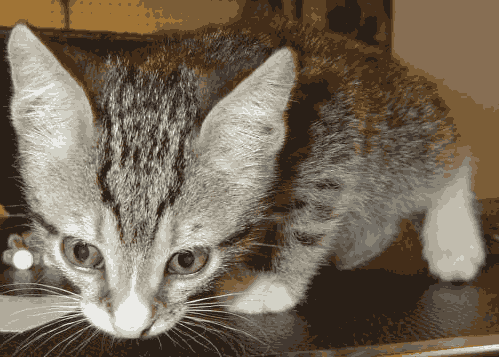
\includegraphics[width=\textwidth]{photos/kmeans_red_16_32}
    \caption{Zdjęcie zredukowane do 16 kolorów po redukcji głębi kolorów pliku (42138 B)}
  \end{minipage}
\end{figure}


\subsubsection{Porównanie rozmiaru doboru kolorów algorytmem k-means i systemowym w zdjęciach zdjęć w formacie .png z redukcją głębi kolorów}

\label{f:red_vs_red}

\begin{figure}[H]
	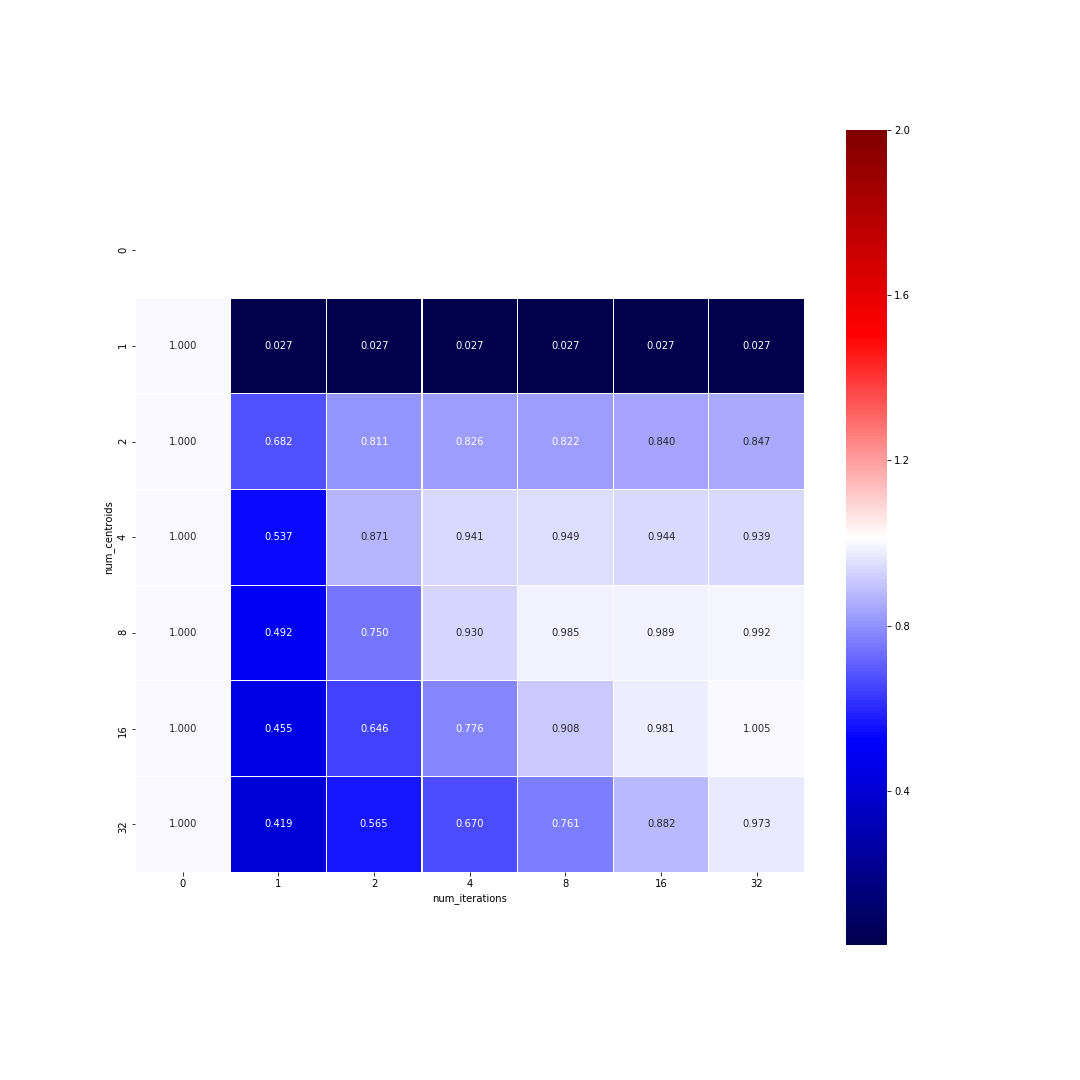
\includegraphics[width=0.9\textwidth]{photos/plots/red_vs_red}
    \caption{Wykres jakości wyników z tabeli \ref{m:red_vs_red}}
\end{figure}

Pierwsza kolumna ($num\_iterations = 0$) to rzecz jasna same wartości $1.0$, gdyż widać w niej porównanie średnich rozmiarów plików uzyskanych poprzez samą tylko systemową redukcję głębi kolorów (bez uprzedniej redukcji kolorów za pomocą k-means) z samymi sobą.

Dalsze kolumny przedstawiają ciekawsze wyniki, z których można wywnioskować, że dobór kolorów algorytmem k-means daje mniejszy lub porównywalny rozmiar zdjęć niż dobór kolorów poprzez narzędzie systemowe.

Co więcej, krótkie badania preferencyjne przeprowadzone na kilku osobach wykazały, że dobór kolorów uzyskiwany za pomocą k-means najczęściej milszy oku i bardziej przypominający oryginał.

\begin{figure}[H]
  \centering
  \begin{minipage}[b]{0.25\textwidth}
    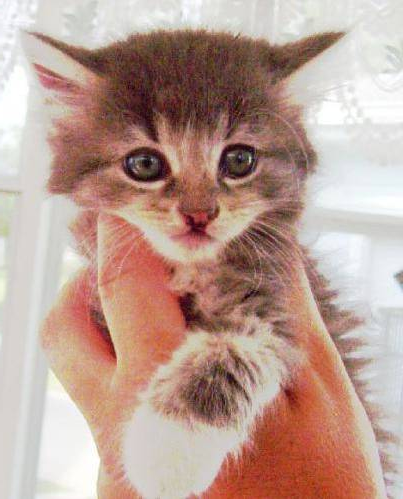
\includegraphics[width=\textwidth]{photos/original}
    \caption{Zdjęcie oryginalne (282801 B)\\\\\\\\}
  \end{minipage}
  \hfill
  \begin{minipage}[b]{0.25\textwidth}
    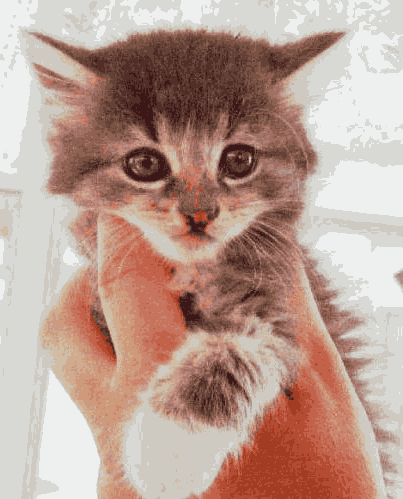
\includegraphics[width=\textwidth]{photos/kmeans_red_32_16}
    \caption{Zdjęcie zredukowane do 32 kolorów przez 16 iteracji k-means po redukcji głębi kolorów pliku (45795 B)}
  \end{minipage}
  \hfill
  \begin{minipage}[b]{0.25\textwidth}
    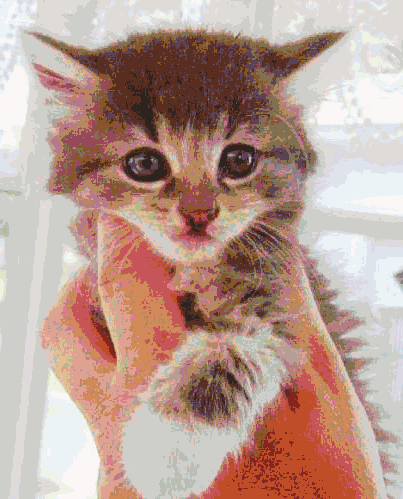
\includegraphics[width=\textwidth]{photos/kmeans_red_32_0}
    \caption{Zdjęcie zredukowane do 32 kolorów wyłącznie poprzez redukcję głębi kolorów pliku (47415 B)}
  \end{minipage}
\end{figure}


\subsubsection{Porównanie obrazów w formacie .png ze zredukowaną głębią kolorów z oryginalnym zdjęciem w formacie .jpg}

\label{f:red_vs_jpg}

\begin{figure}[H]
	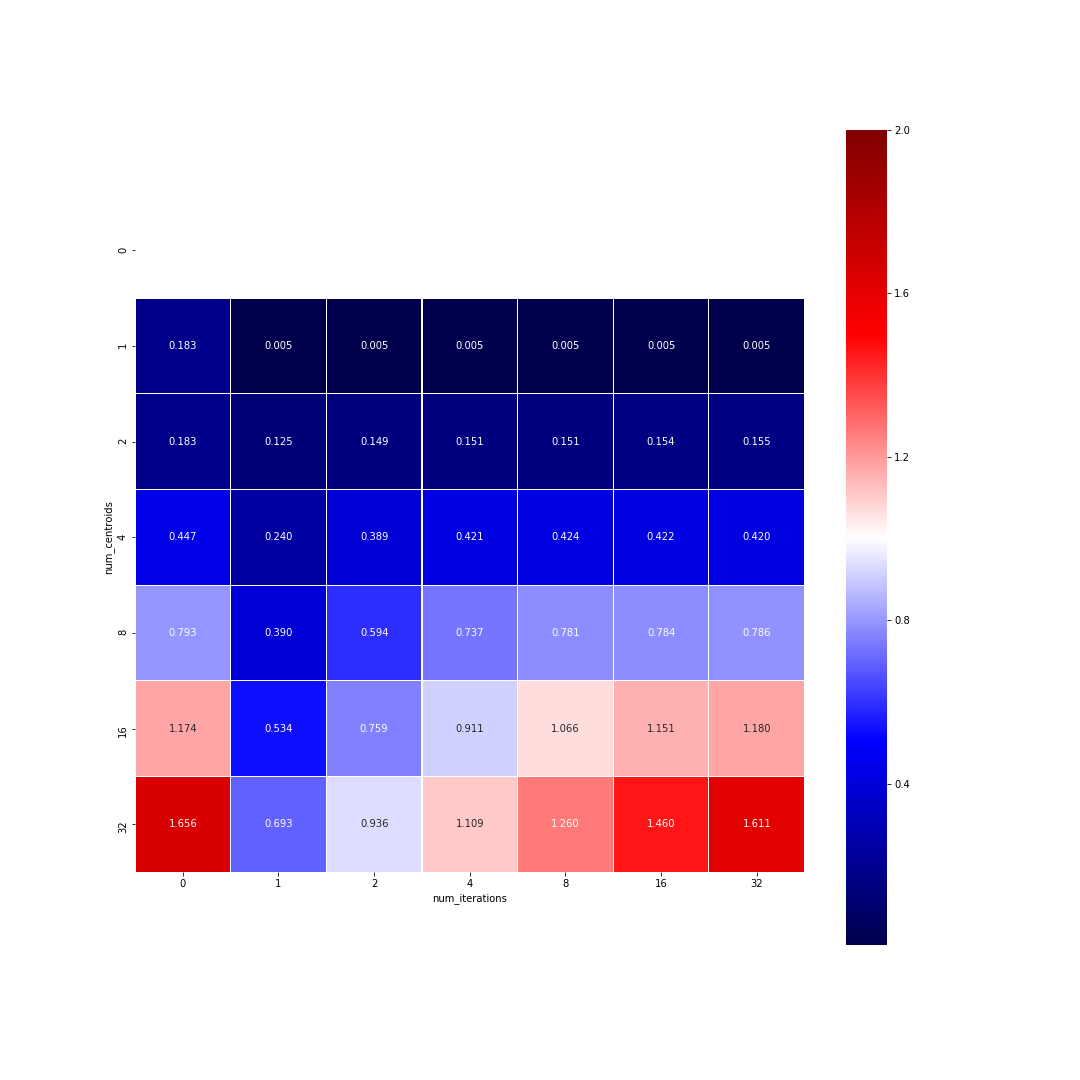
\includegraphics[width=0.9\textwidth]{photos/plots/red_vs_jpg}
    \caption{Wykres jakości wyników z tabeli \ref{m:red_vs_jpg}}
\end{figure}

Widać, że w większości przypadków skompresowane poprzez redukcję głębi obrazy .png mają mniejszy rozmiar niż oryginalny obraz zapisany jako .jpg. Niemniej jednak im lepsza jakość skompresowanego obrazu (więcej kolorów, więcej iteracji), tym bardziej porównanie wychodzi na korzyść oryginalnego .jpg.

\subsection{Wnioski dodatkowe}

Podczas pomiaróœ poczyniliśmy dodatkowe obserwacje:
\begin{enumerate}
\item Algorytm k-means (a przynajmniej nasza jego implementacja) działa dość powoli testowany na laptopie. Jego implementacja np. z biblioteki OpenCV będzie zapewne szybsza.
\item Narzędzie systemowe, choć daje nieco większe i nieco gorsze wizualnie obrazy, działa znacznie szybciej od naszej implementacji k-means.
\end{enumerate}

\section{Podsumowanie}

Podczas naszych badań udało nam się zaimplementować algorytm k-means, który z sukcesem redukuje liczbę kolorów w obrazie. Redukcja kolorów ma pozytywny wpływ na rozmiar obrazu, gdy zapisaujemy go w formacie .png - tego wpływu nie obserwujemy na dłuższą metę gdy zapisujemy obraz w formacie .jpg.

Sprawia to, że sama redukcja kolorów nie przynosi pożądanych skutków - format .jpg osiąga lepsze wyniki od .png rozszerzonego o redukcję.

Użytek ww. narzędzia systemowego, które fizycznie zmniejsza głębię kolorów w plikach .png znacznie poprawia wyniki kompresji. Przy odpowiednio niskiej liczbie kolorów, tak skompresowane pliki .png osiągają mniejsze rozmiary niż oryginalny .jpg oraz pliki .jpg skompresowane analogicznie.

Co więcej, zauważamy że selekcja odpowiednich kolorów za pomocą algorytmu k-means (zamiast kazać to robić narzędziu systemowemu) dodatkowo poprawia działanie narzędzia. Wynikowe obrazy są lepsze wizualnie przy mniejszym lub porównywalnym rozmiarze, co wyniki użycia samego tylko narzędzia.

Ostatecznie jednak udaje się nam uzyskać niższy rozmiar niż pliki .jpg tylko przy niskich liczbach kolorów (wyniki przestają być zadowalające przy 16), do których redukujemy obrazy. Należy sobie zadać pytanie, jaka jest dolna granica liczby kolorów do której redukujemy, przy której obraz wciąż będzie zadowalający wizualnie i nadający się do badania.

Choć nie badaliśmy tego formalnie, to zauważyliśmy że nasza implementacja k-means działa względnie powoli (rząd wielkości sekund), badana na laptopie z procesorem Intel Core i7. Można się tylko spodziewać, że działając na Raspberry Pi 1, czas takiej kompresji obrazów będzie o rzędzy wielkości dłuższy niż zaobserwowany dotychczas.

Rodzi to podejrzenie, czy używając k-means w celu zredukowania zużytej pamięci dyskowej faktycznie zdążymy w praktyce tę pamięć zapełnić. To podejrzenie w połączeniu z powyższymi obserwacjami skłania nas do wybrania w trakcie eksperymentu zapisu w formacie .jpg. Pomimo, że redukcja kolorów ma dobry wpływ na rozmiar obrazu, to w naszym konkretnym przypadku nie znajdujemy dla niej dużego zastosowania.


    \chapter{Kompresja zdjęć metodą SVD}\label{ch:compression}
    \section{Rozkład według wartości osobliwych}\label{sec:compression_svd}

Drugim algorytmem który postanowiliśmy sprawdzić badając kompresję obrazu
był rozkład według wartości osobliwych (SVD - singular value decomposition).
Jeśli każdy piksel potraktujemy jako pojedyńczą wartość (np w skali szarości,
lub systemu pozycyjnego o podstawie 255), to rozkład macierzy pikseli na wartości
osobliwe spowoduje wydzielenie z niech cech bardziej i mniej charakterystycznych,
ponieważ początkowe wartości osobliwe kodują najwięcej informacji. Następnie można
odtworzyć macierz dodając do siebie jedynie część wartości osobliwych. Wówczas zdjęcie
zredukuje swój rozmiar, jednocześnie zachowując najważniejsze szczegóły.

Obrazek testowy poniżej miał 512x512 pikseli, więc możliwe było podzielenie go na 512
wartości osobliwych. W wynikach możemy dostrzec poprawiającą się jakość wraz z rozmiarem
i liczbą wartości osobliwych wziętych pod uwagę. Ciekawym efektem który możemy zaobserwować
w przypadku formatu png, jest spadek rozmiaru przy wszystkich 512 wartościach osobliwych.

\begin{center}
    \begin{longtable}{|l|c|c|}
        \caption{Porównanie przebiegów}\\
        \hline
        \textbf{\thead{Ilość wartości \\ osobliwych}} & \textbf{JPG} & \textbf{PNG} \\
        \hline
        \endfirsthead
        \multicolumn{3}{c}%
        {\tablename\ \thetable\ -- \textit{cd}} \\
        \hline
        \textbf{\thead{Ilość wartości \\ osobliwych}} & \textbf{JPG} & \textbf{PNG} \\
        \hline
        \endhead
        \multicolumn{3}{r}{\textit{cdn}} \\
        \endfoot
        \endlastfoot

        \hline
        org & 
\includegraphics[width=0.4\textwidth]{photos/photo_org.jpg} & 
\includegraphics[width=0.4\textwidth]{photos/photo_org.png} \\
        & 46K & 247K \\
        \hline
        1 & 
\includegraphics[width=0.4\textwidth]{photos/photo_1.jpg} & 
\includegraphics[width=0.4\textwidth]{photos/photo_1.png} \\
        & 14K & 363K \\
        \hline
        5 & 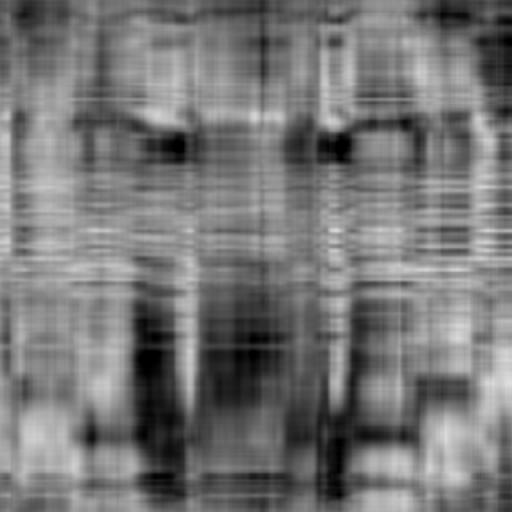
\includegraphics[width=0.4\textwidth]{photos/photo_5.jpg} & 
\includegraphics[width=0.4\textwidth]{photos/photo_5.png} \\
        & 21K & 411K \\
        \hline
        10 & 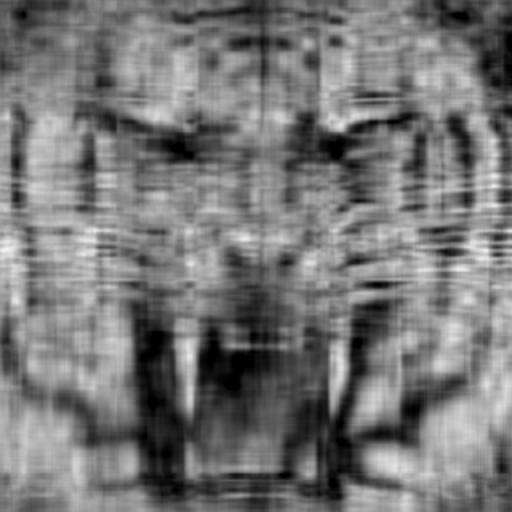
\includegraphics[width=0.4\textwidth]{photos/photo_10.jpg} & 
\includegraphics[width=0.4\textwidth]{photos/photo_10.png} \\
        & 26K & 429K \\
        \hline
        15 & 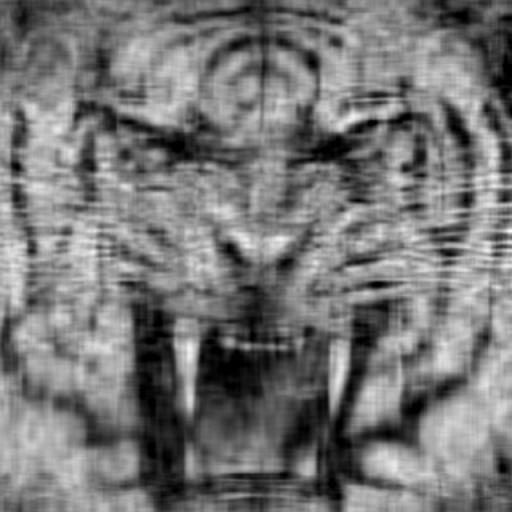
\includegraphics[width=0.4\textwidth]{photos/photo_15.jpg} & 
\includegraphics[width=0.4\textwidth]{photos/photo_15.png} \\
        & 29K & 438K \\
        \hline
        50 & 
\includegraphics[width=0.4\textwidth]{photos/photo_50.jpg} & 
\includegraphics[width=0.4\textwidth]{photos/photo_50.png} \\
        & 39K & 456K \\
        \hline
        100 & 
\includegraphics[width=0.4\textwidth]{photos/photo_100.jpg} & 
\includegraphics[width=0.4\textwidth]{photos/photo_100.png} \\
        & 44K & 464K \\
        \hline
        512 & 
\includegraphics[width=0.4\textwidth]{photos/photo_512.jpg} & 
\includegraphics[width=0.4\textwidth]{photos/photo_512.png} \\
        & 46K & 247K \\
        \hline
    \end{longtable}
\end{center}

Niestety zadawalająca jakość obrazu pojawia się przy ok 20\% oryginalnego obrazu, co daje zmniejszenie
rozmiaru w granicach 5\%. Spadek jakości jest zauważalny i ta numeryczna metoda kompresji nie oferuje
wystarczającego zmniejszenia rozmiaru przy tak znaczącym spadku jakości. Dlatego też ją także odrzuciliśmy.


    \chapter{Geolokalizacja}\label{ch:geolocalisation}
    \section{Wstęp techonologiczny}\label{sec:geolocalisation_introduction}

Aby poznać lokalizację stacji ISS wykorzystujemy technikę telemetrii opartą o TLE (two-line elements).
Dzięki informacjom zawartym w TLE, można przy użyciu specjalnych programów komputerowych
(np pakiet ephem dostępny w języku programowania Python do wersji 3.4 włącznie)
wyznaczyć dokładne położenie danego satelity w czasie i przestrzeni.

TLE to najbardziej popularny format zapisu elementów orbitalnych sztucznych satelitów Ziemi.
W systemie TLE, w postaci dwóch linii (wierszy) zapisane są parametry keplerowskie orbit
sztucznych satelitów oraz inne informacje takie jak numer satelity w katalogu USSPACECOM
i NORAD, daty wprowadzenia satelity na orbitę i wygenerowania informacji TLE.

\noindent \textit{
\\
ISS \\
1 25544U 98067A 18019.53562654 .00016717 00000-0 10270-3 0 9002 \\
2 25544 51.6396 39.7742 0003526 27.0102 333.1234 15.54187636 15395 \\
}

W systemie tym zawarte są kepleriańskie parametry orbit, czyli orbit stałych (przewidziane
są konkretne zmiany orbity względem czasu). Nieregularności orbitalne sztucznych satelitów,
spowodowane są m.in. wiatrem słonecznym, tarciem atmosferycznym i nieregularnym polem
magnetycznym na różnych szerokościach geograficznych Ziemi. Dlatego elementy orbitalne TLE,
należy często uaktualniać gdyż z biegiem czasu stają się niedokładne i błędnie odzwierciedlają
położenie satelity w przestrzeni. Częściej należy uaktualniać TLE satelitów o niskich orbitach
sięgających do 400 km wysokości (np. ISS) - zaleca się aktualizację co 1-2 tygodnie. TLE satelitów
o wyższych orbitach można uaktualniać odpowiednio, co kilka tygodni, a nawet miesięcy.
System zapisu jest powszechnie używany przez NASA i NORAD, które na bieżąco podają nowe
efemerydy zapisywane w systemie TLE.

Mając dokładną lokalizację stacji ISS w danej chwili możemy oznakować zdjęcie koordynatami
geograficznymi punktu na Ziemi znajdującego się dokładnie pod stacją.

\section{Wyznaczanie horyzontu}\label{sec:geolocalisation_horizon}

Postanowiliśmy dodatkowo wyznaczyć widoczny ze stacji obszar w granicach horyzontu, by lepiej
orientować się w możliwościach kamery znajdującej się na ISS.

Punkt reprezentujemy jako parę współrzędnych wyrażonych w stopniach dziesiętnych (DD - Decimal degrees).
Nie wiedzieć czemu, przyjęło się że we współrzędnych najpierw określamy szerokość (N, S),
a dopiero potem długość (W, E) - odwrotnie niż na układzie współrzędnych.
Ponieważ operujemy w geometrii sferycznej, wzory znane z geometrii euklidesowej nie mają
tutaj zastosowania. W szczególności odległość dwóch punktów o tej samej różnicy drugich współrzędnych,
jest różna i zależy także od pierwszej współrzędnej.

Dzieje się tak, ponieważ reprezentacja w stopniach dziesiętnych zakłada, że mapa jest prostokątna, a
sfery nie da się spłaszczyć bez dodatkowych, zaburzających proporcje mapy operacji. Sferę rozcina
się na płatki (sphere net, gores), i dokonuje ich projekcji i uzupełnienia brakujących fragmentów.

\begin{center}
    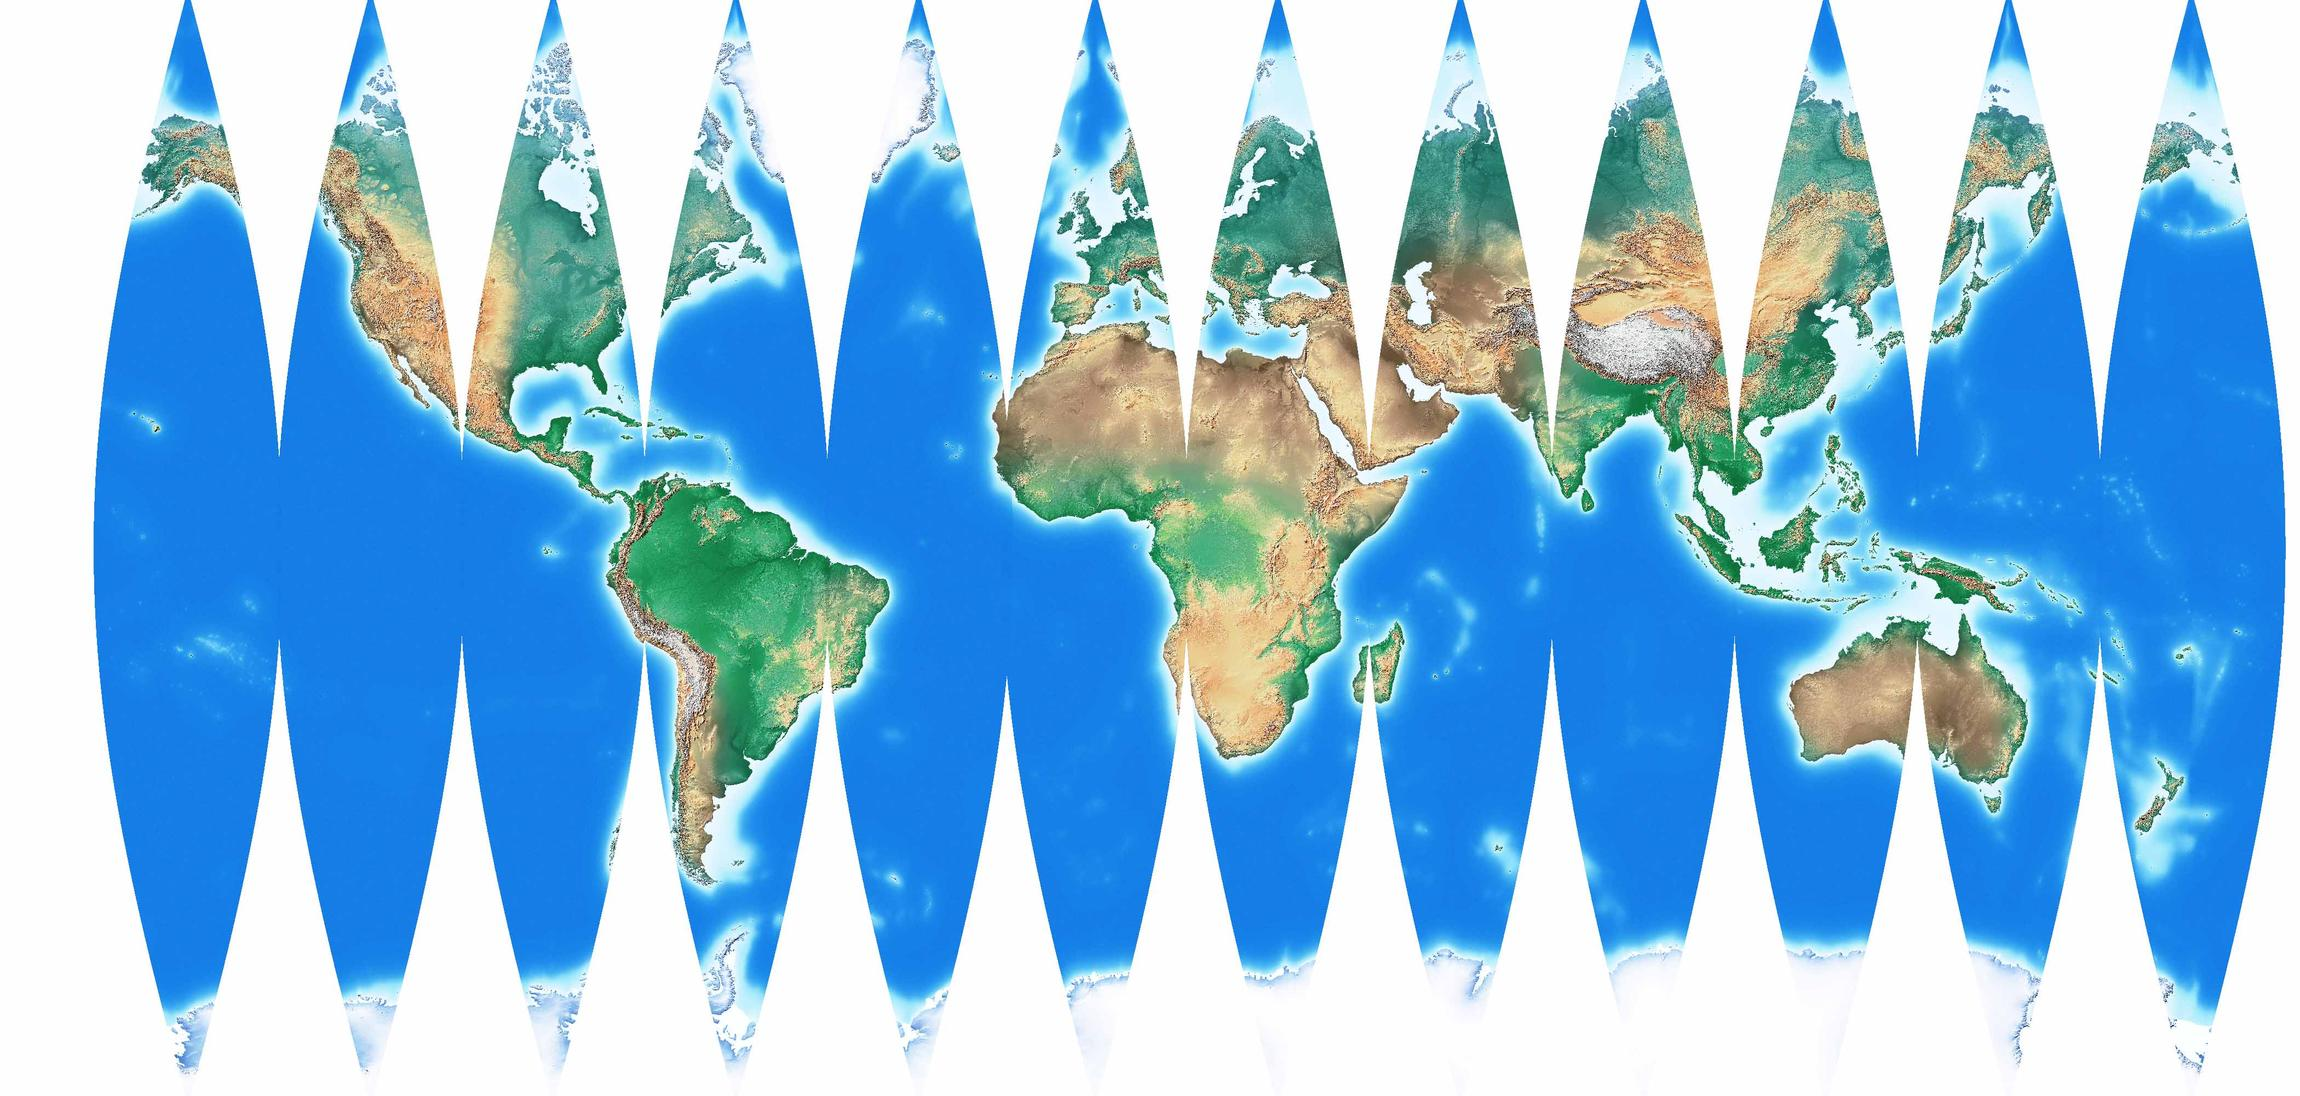
\includegraphics[width=0.9\textwidth]{photos/gores_map.jpg}
    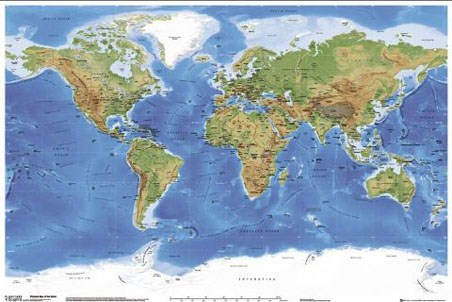
\includegraphics[width=0.9\textwidth]{photos/full_map.jpg}
\end{center}

Naszym celem było wyznaczenie okręgu na sferze, którego środek wypadałby w punkcie bezpośrednio
pod stacją ISS, a obwód wyznaczał horyzont. Okrąg ten chcieliśmy przybliżać wielokątem foremnym.
Ponieważ rozważaliśmy także automatyczne wyznaczanie jakie kraje są widoczne ze stacji w danej
chwili, zdecydowaliśmy się na podział wielokąta na nachodzące na siebie częściowo prostokąty
(by móc sprawdzać czy punkt tworzący granicę kraju jest wewnątrz wielokąta sprawdzalibyśmy czy
zawiera się w którymś z prostokątów).

\begin{figure}[H]
    \begin{subfigure}{0.5\textwidth}
        \centering
        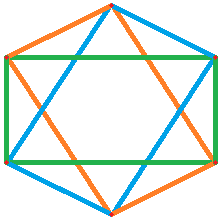
\includegraphics[width=0.9\linewidth]{photos/circle.png}
        \caption{Przykładowy podział wielokąta foremnego na nachodzące prostokąty}
    \end{subfigure}
    \begin{subfigure}{0.5\textwidth}
        \centering
        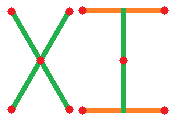
\includegraphics[width=0.9\linewidth]{photos/models.png}
        \caption{Możliwe metody budowania prostokątów}
    \end{subfigure}
\end{figure}

Znaleźliśmy dwa możliwe sposoby modelowania prostokątów, prowadząc z punktu obie przekątne, lub
prowadząc linię równoległą do boków, a później dwie linie prostopadłe do niej. Myśląc także o
innych zastosowaniach naszych algorytmów (np wyznaczania prostokątnego ograniczenia jakiejś
prostej na mapie) zdecydowaliśmy się początkowo na metodę drugą, co ostatecznie okazało się błędem.

\section{W geometrii euklidesowej}\label{sec:geolocalisation_euclidean}

Początkowo, nie zdając sobie sprawy z problemu geometrii sferycznej, zastosowaliśmy twierdzenia
Pitagorasa i wzór na funkcję liniową, by wyznaczyć kolejne prostokąty. Poniższe grafiki przedstawiają
wizualizację punktów w Google Earth. Na pierwszej z nich możemy zaobserwować, że mimo przesunięcia
na górze i na dole o tyle samo punktów dziesiętnych, otrzymaliśmy trapez, a nie prostokąt. Wynika
to z uzupełniania i rozciągania mapy przy spłaszczaniu sfery. W małej skali (gdzie odległości miedzy
punktami wynosiły kilka metrów) otrzymywaliśmy równoległobok, zamiast prostokąta.

Wymyśliliśmy, że możemy przed zastosowaniem operacji znanych z geometrii euklidesowej przeskalować
współrzędne x punktów wejściowych, tak, by kąt prosty był tam, gdzie się go spodziewamy. Po
zastosowniu tych operacji nowe punkty mogliśmy przeskalować odwrotnie. Spodziewaliśmy się
otrzymać prostokąty, nie trapezy. W małej skali (gdy odległości między punktami wynosiły kilka metrów)
wynik był faktycznie znacznie lepszy niż wcześniej. W dużej skali jednak wyniki były jeszcze gorsze, co
widać na drugim obrazku. Punkty były od siebie oddalone o tyle, że każdy z nich musiałby być przeskalowany
przez inną wartość, co psuło ideę naszego pomysłu.

\begin{figure}[H]
    \begin{subfigure}{0.59\textwidth}
        \centering
        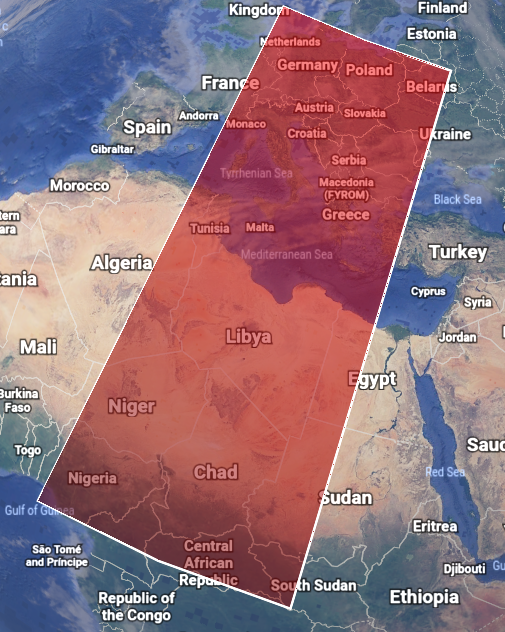
\includegraphics[width=0.9\linewidth]{photos/method1.png}
        \caption{Po zastosowaniu wzorów z geometrii euklidesowej}
    \end{subfigure}
    \begin{subfigure}{0.41\textwidth}
        \centering
        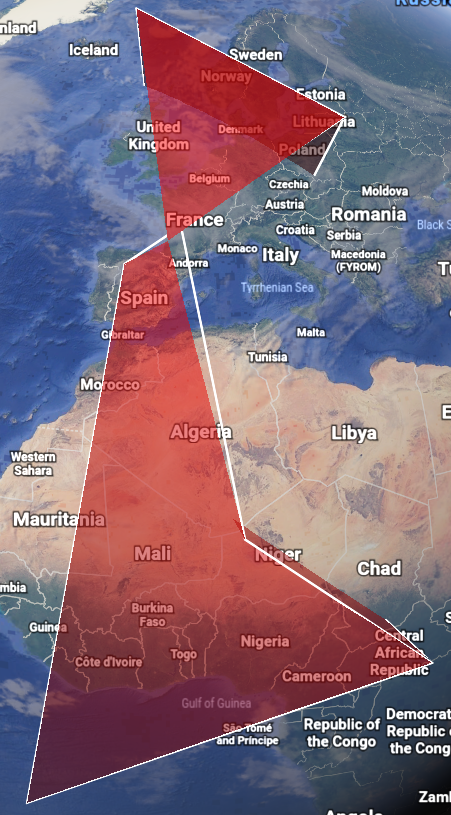
\includegraphics[width=0.9\linewidth]{photos/method2.png}
        \caption{Po wcześniejszym skalowaniu}
    \end{subfigure}
\end{figure}

\section{W geometrii sferycznej}\label{sec:geolocalisation_spherical}

Porzucilismy pomysł korzystania ze znanych nam wzorów i wyszukaliśmy odpowiadające im wzory
w geometrii sferycznej. Pomocna okazała się \href{http://www.movable-type.co.uk/scripts/latlong.html}{ta strona}.

$
\\
\text{W szczególności:} \\
newlat = \arcsin(\sin(lat) \cdot \cos(d) + \cos(lat) \cdot \sin(d) \cdot \cos(bearing)) \\
newlon = lon + \arctan(\sin(bearing) \cdot \sin(d) \cdot \cos(lat), \cos(d) - \sin(lat) \cdot \sin(newlat)) \\
\text{gdzie:} \\
d - \text{odległość do szukanego punktu} \\
lat, lon - \text{współrzędne punktu startowego} \\
bearing - \text{kąt skierowany przeciwnie do wskazówek zegara} \\
\text{między prostą skierowaną na północ i prostą łączącą oba punkty} \\
$

Pozwoliło to znacząco poprawić osiągane wyniki, co można zaobserwować na pierwszej grafice
poniżej. Niestety Wielokąt wciąż nie był idealny. Występowały na nim 'ząbki' wynikające z
różnic rozszerzaniu poszczególnych prostokątów.

Wówczas przypomnieliśmy sobie o drugiej możliwoście generowania prostokątów - bezpośrednio
z przekątnych - co ostatecznie pozwoliło uzyskać porządany od początku wynik.

\begin{figure}[H]
    \begin{subfigure}{0.5\textwidth}
        \centering
        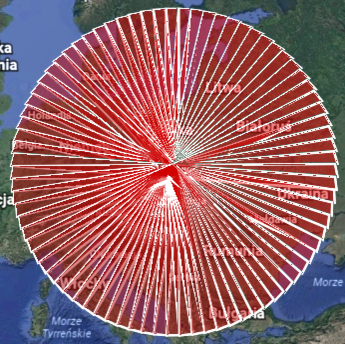
\includegraphics[width=0.9\linewidth]{photos/method3.png}
        \caption{Po zastosowaniu wzorów sferycznych}
    \end{subfigure}
    \begin{subfigure}{0.5\textwidth}
        \centering
        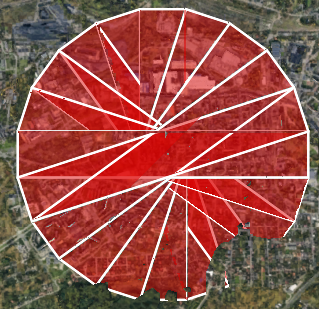
\includegraphics[width=0.9\linewidth]{photos/method4.png}
        \caption{Po zmianie metody budowania prostokątów}
    \end{subfigure}
\end{figure}

ESA poinformowało nas później, że nie jesteśmy w stanie fotografować ze stacji całego widocznego
horyzontu, a jedynie obszar bezpośrednio widziany z okna w którym umiejsciowiony jest mikrokomputer
Raspberry, więc ostatecznie nie wykorzystaliśmy tych obliczeń. Uważamy jednak że poświęcony czas
nie poszedł na marne, nauczyliśmy się bardzo dużo o geometriach nieeuklidesowych.


    \chapter{Ostateczna wersja programu}\label{ch:final}
    \section{Ostatnie problemy}\label{sec:final_introduction}

Po upewnieniu się, że kompresja stosowana w formacie jpg jest bezkonkurencyjna,
oraz zbadaniu, jak w odpowiedni sposób możemy pobierać lokalizację stacji kosmicznej,
musieliśmy zmierzyć się z ostatnim problemem. Chcielismy dane o czasie wykonania
zdjęcia i położeniu stacji zapisywać w nazwie zdjęcia, jednak ESA poinformowało
nas, że nazwy plików mogą zostać zmienione w trakcie pobierania przez nich danych.
Musieliśmy wymyślić sposób, by móc jednoznacznie przyporządkować zdjęcie do daty
i lokalizacji.

Wymyśliliśmy trzy sposoby rozwiązania tego problemu:
\begin{itemize}
    \item zapisanie danych w metadanych zdjęcia - odrzuciliśmy to rozwiązanie, ponieważ
    ESA zmieniając nazwę pliku, mogła zmieniać również metadane - rozwiązanie było niepewne
    \item zapisanie danych na zdjęciu - odrzucone, ponieważ po pierwsze mogliśmy zastąpić
    potencjalnie ważny fragment zdjęcia, a po drugie odzyskanie tych danych mogłoby być
    trudne algorytmicznie
    \item haszowanie zdjęcia i zapis do pliku csv wartości hash, daty i lokalizacji -
    zdecydowaliśmy się na to rozwiązanie
\end{itemize}

\section{I ich rozwiązania}\label{sec:final_conclusion}

Musieliśmy także rozważyć, jak często wykonywać zdjęcia, by zająć jak najmniej miejsca na
karcie pamięci, a jednocześnie nawet po odrzuceniu niewyraźnych zdjęć mieć sfotografowany
cały możliwy obszar. Obliczyliśmy, że jeden piksel zdjęcia odpowiada 161 metrom na Ziemi,
a ISS porusza się z prędkością odpowiadającą przesunięciu o połowę widocznego na zdjęciu
obszaru w ciągu pół minuty. Ostatecznie zdecydowaliśmy się na wykonywanie zdjęć co 15 sekund.

Obecnie, po wielu próbach i błędach czekamy na wyniki działania naszego kodu na Międzynarodowej
Stacji Kosmicznej i przygotowujemy algorytmy uczenia maszynowego, które wykorzystamy do analizy
zebranych zdjęć.


\end{document}
